\documentclass[fleqn]{homework}
\usepackage{gensymb}
\usepackage{hyperref}
\usepackage{float}
\usepackage{graphicx}
\usepackage{caption}
\usepackage{subcaption}
\usepackage{multirow}
\usepackage{amsmath}
\usepackage{relsize}
\usepackage{float}
\usepackage{amssymb}
\usepackage[font={small,it}]{caption}

% The title is the title of the homework
\title{Machine Learning 2016-2017: project report}
% Here you specify which course the homework is for
\course{Machine Learning 2016-2017}
% This is you
\author{Stijn Decubber}
% This is the number of the homework. You don't have to specify it.
\hnum{}
%If you don't specify a date, the date that is used will be the date of today
%\date{34 october 3012}

% Verbatim code: \begin{verbatim} code \end{verbatim} 
% Code listing: \begin{lstlisting} code \end{lstlisting}
% Labelled equation: \begin{equation}\label{lab} equation \end{equation}
% Equation array: \begin{eqnarray}\label{lab} equation1 \\ equation2 \end{eqnarray}
% Figures: %\begin{figure}[htbp]
	%\centering
		%\includegraphics[width=0.50\textwidth]{IntroLatexFigure.pdf}
	 %\caption{Name of Figure}
	%\label{fig:IntroLatexFigure}
%\end{figure}

\begin{document}
I work as a PhD student on a project that aims at quantifying the impact of climate extremes such as droughts and heat waves on vegetation, to improve our understanding of how future climate change might affect vegetation. To this end, we use observational time series data on climate (temperature, vegetation, soil moisture etc.) and on vegetation, obtained from satellites. 

I considered using the data from my PhD for this project for the course of Machine Learning. However, I came to the conclusions that 1) the research questions that we try to answer are statistical inference problems and not prediction problems and 2) the nature of the data (spatio-temporal multivariate time series) is not really suited to fit complex machine learning models \footnote{I tried a couple of models that take the spatial aspect of the data into account, but the data between neighbouring pixels is heavily correlated so spatial information is basically redundant.}.

Therefore, I decided to participate in a Kaggle competition and to describe my approach in a report for the project of this course. Another reason to participate was that the competition is related to the topic of my PhD, so it was a nice opportunity to learn about machine learning on a different data set. I participated together with a colleague, and we ended up at the 41th place on the private leaderboard (top 5\%). 
\section{Data and goal of the competition}

The problem at hand is a multi-label classification problem, with satellite imagery from the Amazon rainforest as input data. The goal is to label images with one or more of seventeen possible labels. The labels can be divided in three large subsets:
\begin{itemize}
\item{Weather labels: cloudy - partly cloudy - haze - clear}
\item{Common labels: primary forest - water - habitation - agriculture - road - cultivation - bare ground}
\item{Rare labels: slash and burn - logging - blooming - conventional mining - 'artisinal' mining - blow down}
\end{itemize}

While each image can be associated with multiple labels, some labels are mutually exclusive. For instance, an image that is 'cloudy' should not be associated with any other label. Figure \ref{labels} shows the occurrence of each label in the training set. Clearly, some labels occur very frequently ('clear' and 'primary'), while others are extremely rare, with only about 100 training examples for the rarest labels. Figure \ref{cooc} visualizes the co-occurence matrix of the 17 labels. Again, the combination 'primary clear' pops out as the most frequently occurring label combination. There are clear dependencies between labels and only 458 unique label combinations occur in the training data, out of $2^{17}$ theoretically possible combinations. Figure \ref{images} shows some example images with the associated labels from the training set.

For the competition, there were 40479 labeled training images and 61191 testing images for which predictions had to be submitted to Kaggle. The public and private leaderboards were calculated with 66\% and 34\% of the test data, respectively. The training images were hand-labeled and there was some label noise to be expected. The images were provided as 3-channel (RGB) jpg-files of size 256x256 pixels. Additionally, the same images were provided as 4-channel tiff-files (additional near-infrared channel). We decided to work with the 3-channel jpg images because there seemed to be a mismatch between the jpg and the tiff images, as well as for for computational considerations.

\begin{figure}[H]
	\centering
     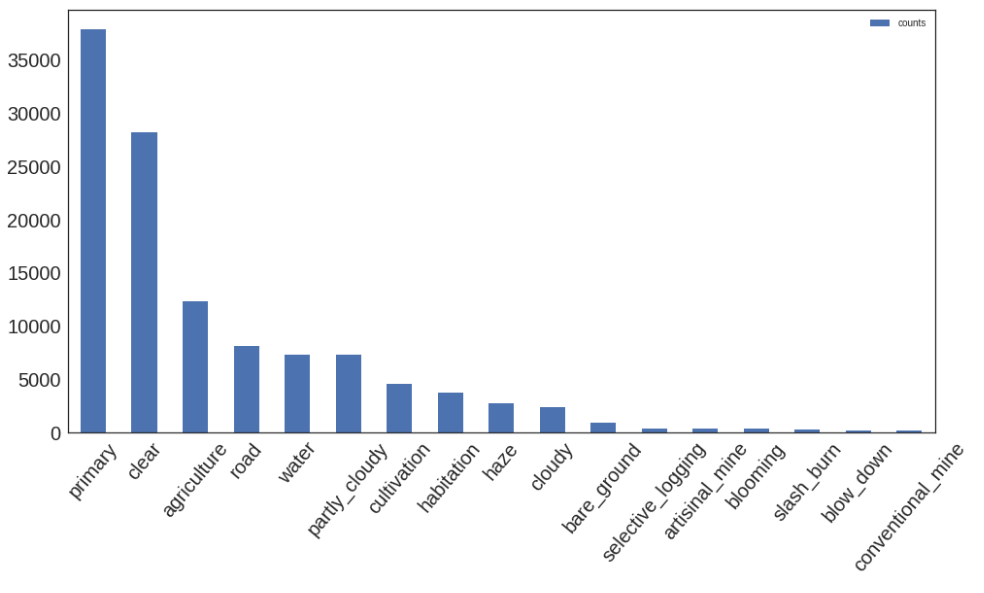
\includegraphics[width=0.7\linewidth]{figures/labels.png} 
	\caption{Label distribution. There is a clear imbalance in frequence of the different labels.}
	\label{labels} 
\end{figure}

\begin{figure}[H]
	\centering
     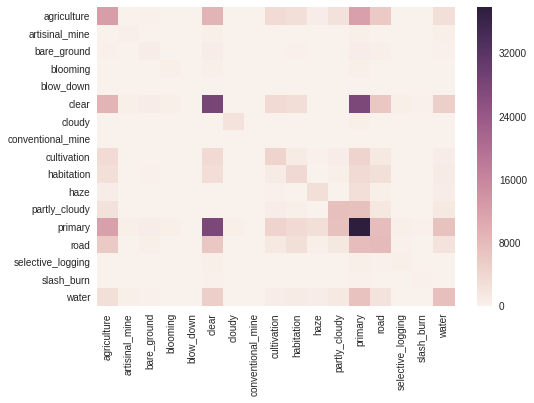
\includegraphics[width=0.7\linewidth]{figures/cooc1.png}
	\caption{Label co-occurence matrix. Some labels frequently occur together with other labels, while others are mutually exclusive. }
	\label{cooc} 
\end{figure}

\begin{figure}[H]
	\centering
     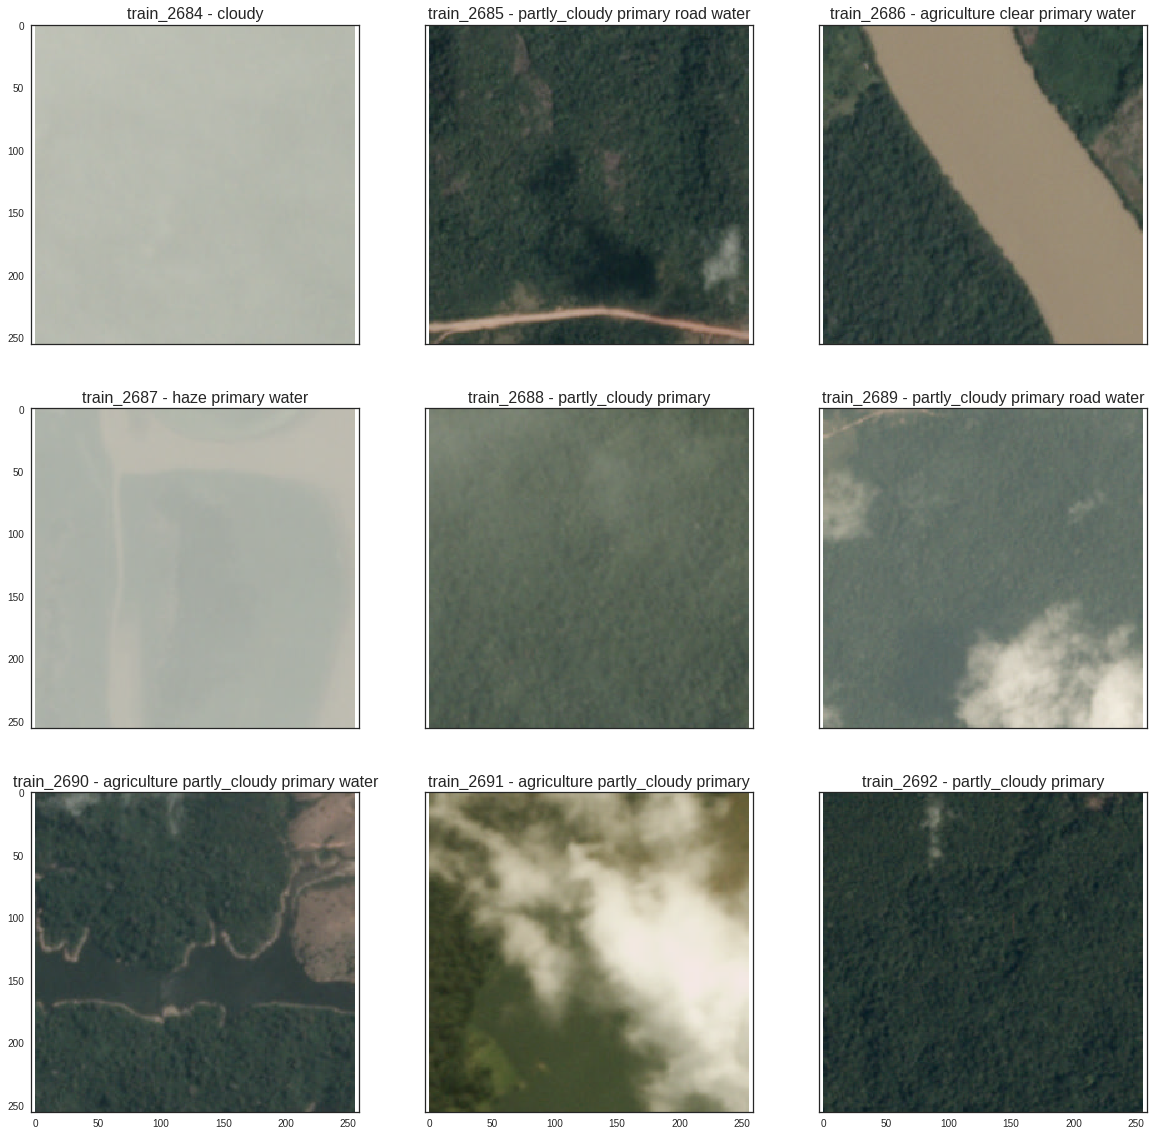
\includegraphics[width=0.9\linewidth]{figures/images.png}
	\caption{Some example images from the training data set.}
	\label{images} 
\end{figure}

\section{Evaluation metric}
The $F_2$ score was used to evaluate the predictions. Generally, the $F_{\beta}$ score is a weighted harmonic mean between precision and recall. Precision $p$ is the ratio of true positives to all predicted positives (how accurate are the positive predictions?) and recall $r$ is the ratio of true positives to all actual positives (how much of the positives were detected?). The $F_{\beta}$ score is then given as:

\begin{equation}\label{Fscore}
F_{\beta} = (1+\beta^2)\frac{pr}{\beta^2p+r}, \ p = \frac{tp}{tp+fp}, \ r = \frac{tp}{tp+fn}
\end{equation}
By multiplying precision with a factor 4 ($\beta = 2$) in the denominator of \ref{Fscore}, the $F_2$ score penalizes false negative predictions (lower recall) more than it does false positive predictions (lower precision). For this competition, the $F_{2}$ score is calculated for each sample separately and averaged all the samples in the test dataset. 

\section{Data processing and models}
After playing around with tree-based methods (random forests, XGBoost) using RGB-histogram statistics as features, we decided to go for convolutional neural networks (CNNs) since they are know for their strong performance on tasks with image data. Therefore, no hand-crafted features were constructed. We experimented with different CNN architectures and training schemes, which will be discussed further on. A particular point of attention was the F-score metric. The $F_{\beta}$ score is not a differentiable loss function. The most common way to cope with this is to use a surrogate loss function such as the binary cross-entropy for multi-label classification to allow for a network that can be backpropagated through to compute gradients. We considered a second, probabilistic optimizer that has been shown to be Bayes-optimal for multiclass classification problems \footnote{Waegeman, W., Dembczyńki, K., Jachnik, A., Cheng, W., and Hüllermeier, E. (2014). On the bayes-optimality of F-measure maximizers. The Journal of Machine Learning Research, 15(1), 3333-3388.} and implemented it on top of convolutional neural networks. Both approaches will be discussed further on.

We used both Keras (TensorFlow backend) and PyTorch to run our models.

\subsection*{Data processing}

The images were loaded as tensors of shape 256x256x3 and either rescaled between 0 and 1 or standardized with the mean and standard deviation of the imagenet dataset in case pretrained networks were used. Initially, we downsized the images to resolutions as small as 32x32 pixels to debug our code and test different architectures. The best performing final models were trained on 128x128, 224x224 or 256x256 images. 
\subsection*{CNN architectures}
\subsubsection*{A. Custom architecture}

At first, we experimented with a custom architecture that was inspired by a winning CNN architecture in a previous Kaggle competition, also with satellite imagery and which other competitors had been discussing for this competition. The architecture is a part of a U-Net-architecture which is used for image segmentation (classification on the pixel level). A U-Net consist of a downsampling part and an upsampling part (which makes for the U-shape when presented schematically, see below). In the downsampling part, the input images are sequentially downsampled via max pooling to a large number of low-resolution feature maps. In the upsampling part, these high-dimensional small feature maps are upsampled again to obtain a high-resolution output segmentation map with a single channel. Also, the output of each convolutional block in the downsampling is copied and passed on to the upsampling part.

Because the problem in this competition was not a segmentation problem, we used only the first half of this architecture. The upsampling part was replaced with a couple of dense layers, with global average pooling on the intermediary outputs of the convolutional blocks. The idea of passing intermediate output to the final layers is that in this way, both 'global' features learned on a large resolution (such as cloudiness) as well as more specialized local features learned in the later convolutional blocks can be used. The final layer consisted of 17 output nodes with sigmoid activation functions, one node for each of the 17 possible labels. Figure \ref{UNet} shows a U-Net architecture on the left and the model architecture that we used in this competition on the right. In addition, we experimented with batch normalization in between the different layers and with dropout regularization.

\begin{figure}[H]
\centering
   \begin{subfigure}{0.48\linewidth}
      \centering
	  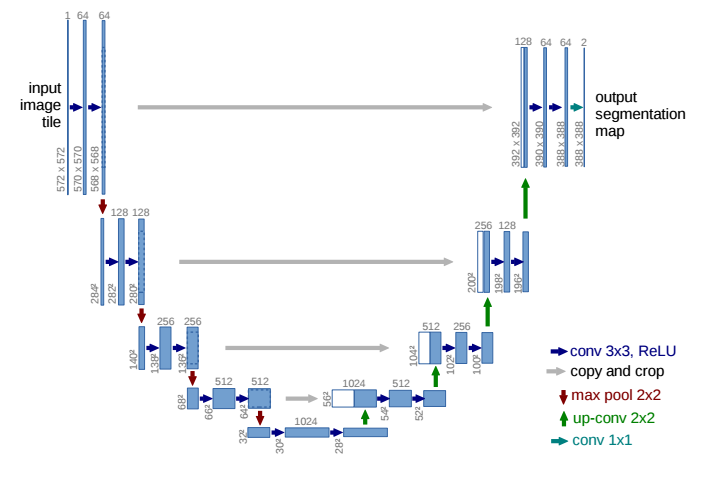
\includegraphics[width=1\linewidth]{figures/UNet.png}
      \caption{}
   \end{subfigure}
   \begin{subfigure}{0.48\linewidth}
      \centering
	  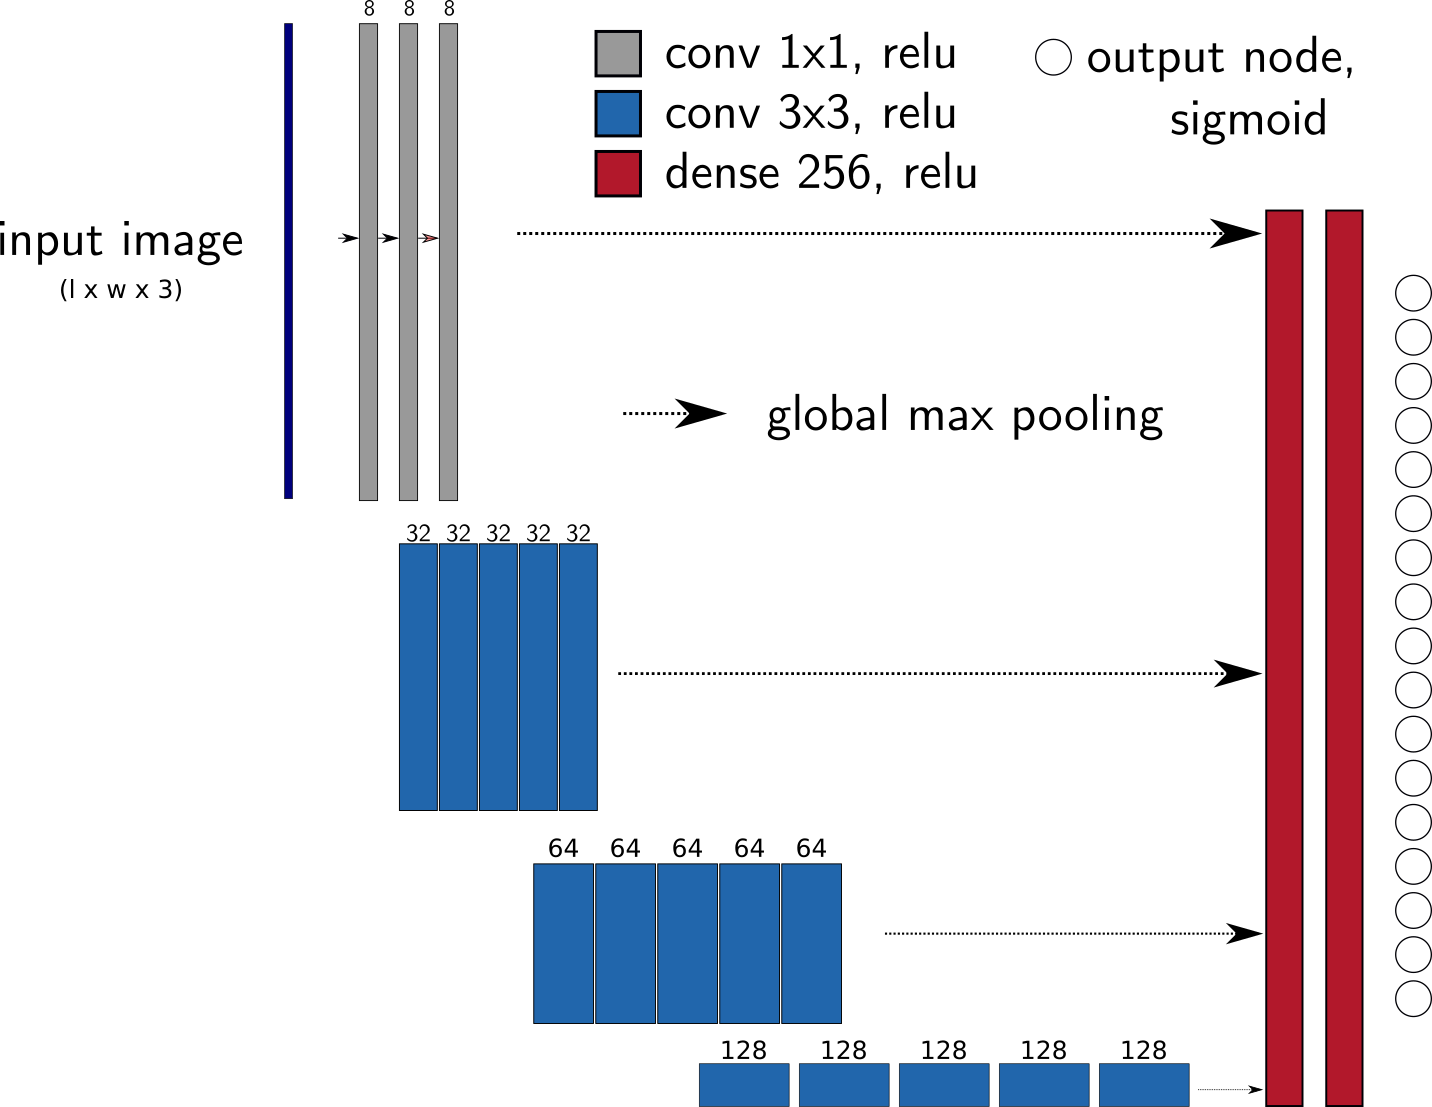
\includegraphics[width=1\linewidth]{figures/Simplenet.png}
      \caption{}
   \end{subfigure}
  \caption{Left: U-Net architecture. Right: CNN architecture used for this competition.}
	\label{UNet} 
\end{figure}

\subsubsection*{B. Pretrained models}

With this convolutional architecture, we obtained public leaderboard scores around 91.5. However, it became clear that most other competitors were using large models that are available online together with pretrained weights, typically on ImageNet, rather than custom architectures. Therefore, we decided to switch to this approach as well. The downside of finetuning these pretrained models was the very large computational cost. Among the models that we used are ResNet50, DenseNet and VGGNet16.

The only change that had to be made to these architectures was the output layer. To do so, we removed the top layer and replaced it with the 17-node output layer suitable for multi-label classification. In order to initialize this final layer with proper weights, we first obtained the output feature maps from the convolutional parts of the models, and used these to pre-train the final multi-label classification layer. The weights obtained as such were used to initialize this output layer after adding it on top of the convolutional architectures.

\subsubsection*{C. Loss function and hyperparameter optimization}
The final output layer of the CNNs consists of 17 neurons with sigmoid activations. Because multiple layers can occur for each instance, the binary cross-entropy loss was used as a loss function, which is suitable for multi-label classification problems. The total loss of the network is then just the sum or the average of the cross-entropy losses over the 17 output nodes.

Before switching to large pretrained architectures, we experimented with different configurations of the custom network presented in Figure \ref{UNet} with more or less convolutional blocks, more or less aggressive dropout, hyperbolic tangent and sigmoid activations instead of relu... With the pretrained networks, we did not have the computational to do a grid search or random search for optimal hyperparameters. We used both stochastic gradient descent with momentum and Adam as optimization algorithms. The pretrained models were trained with a small learning rate (1e-5) to allow a finetuning of the pretrained weights rather than training from scratch. Learning rate annealing was used to decrease the learning rate by a factor of 10 after the validation loss had reached a plateau. 

\subsection*{Train-validation splitting and early stopping}
The training dataset consisted of 40479 images. In order to avoid overfitting on the training data, we split this training data into a training and validation set according to a 90\%-10\% split. This was a trade-off between using enough validation data for the validation set to be representative of the test data, and not losing too much training data. We did not use k-fold cross-validation for computational reasons. The train-validation splitting was done in a random fashion and was redone for training every separate model.

In order to avoid overfitting, we used early stopping by monitoring the loss decay on the validation data. Model training was stopped if the validation loss did not decrease for 5 consecutive epochs, after which the model weights at the start of these 5 epochs was retained as the final model. 

\subsection*{Data augmentation (DA), test-time augmentation (TTA) and pseudo-labeling}

As per standard practice in CNN competitions, we used data augmentation and test-time augmentation to introduce meaningful noise into the images and make our models more robust. We used random horizontal and vertical flips and also small random shifts in both directions. We did not use too aggressive DA such as 45\degree -rotations or random crops in order to avoid the introduction of too much noise and mis-labeled images (for instance, a road occurring in the corner of an image could disappear with a heavy rotation). 

We used the same augmentation schemes to do test-time augmentation: we randomly transformed each test image 10 times and averaged the predictions to come to a final prediction for each test instance. 

Finally, towards the end of the competition we experimented with 'pseudo-labeling' to increase the size of our dataset. We added the test-set images for which labels we had a large consensus amongst our previous highest-scoring submissions to the training set. The idea here is that this consensus prediction is likely to be the ground truth, so these images can be used as training data as well. Using pseudo-labeling allowed us to reach a public LB score larger than 0.93 with a single, non-ensembled model.

\subsection*{F-score optimization}
\subsubsection*{A. Optimal thresholding}
One way to optimize the $F_2$-score is by searching for optimal cut-off thresholds for the predicted probabilities to assign labels to an image instead. The default threshold in binary classification is a probability of 0.5; if the predicted probability exceeds this threshold then the class is presented to be present. In order to optimize the $F_2$-score, a different threshold for each label can be considered. In addition, it will pay off to choose a lower threshold than 0.5 since the $F_2$-score favors false positives over false negatives. We tried both line search (where a threshold is found for each label separately, in a sequential way) and a hill-climbing optimization algorithm (BFGS) on a differentiable approximation of the $F_2$-score to search for the optimal threshold vector in a joint way. Searching for the optimal threshold vector in a joint way yielded slightly better results, albeit at a higher computational cost. Each time, the hill-climbing algorithm was run several times with different initial values, drawn from a $\beta_{5,2}$ distribution (see Figure \ref{beta}) to incorporate the prior knowledge that optimal thresholds should be lower than 0.5 and to speed up convergence. The best performing threshold set was retained for making predictions on the test set. All this was done on the training data, to avoid overfitting on the validation data set. 

\begin{figure}[H]
	\centering
     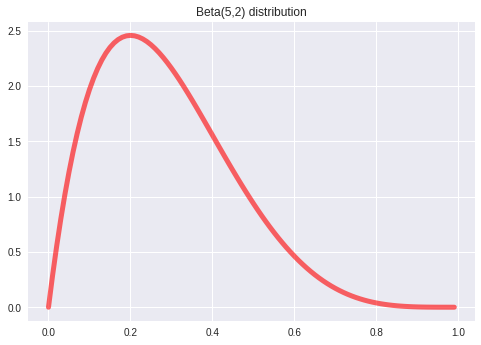
\includegraphics[width=0.4\linewidth]{figures/beta.png}
	\caption{Starting values for the thresholds were sampled from a Beta(5,2) distribution to reinitialize the hill-climbing algorithm several times to find the optimal thresholds.}
	\label{beta} 
\end{figure}

\subsubsection*{B. General F-measure Maximizer (GFM)}
Another way to optimize the $F_2$ score is the GFM-algorithm  \footnote{Waegeman, W., Dembczyńki, K., Jachnik, A., Cheng, W., and Hüllermeier, E. (2014). On the bayes-optimality of F-measure maximizers. The Journal of Machine Learning Research, 15(1), 3333-3388.} \footnote{Dembczynski, K., Jachnik, A., Kotlowski, W., Waegeman, W., and Hüllermeier, E. (2013, February). Optimizing the F-measure in multi-label classification: Plug-in rule approach versus structured loss minimization. In International Conference on Machine Learning (pp. 1130-1138).}. The GFM-algorithm is a probabilistic plug-in rule algorithm for F-measure maximization that requires the estimation of a set of parameters of the joint distribution of the labels conditional on the data. More specifically, the GFM-algorithm takes the following probabilities as input to produce Bayes-optimal predictions (for a given instance):
\begin{equation}\label{GFM}
p_{is} = P(y_i = 1, \mathbf{s_y} = s|\mathbf{x}), \ \ i, s \in \{1,...,m\}
\end{equation}

These probabilities constitute an $m \times m$-matrix $P$, with $m$ the number of labels (17). $\mathbf{s_y}$ is the number of labels present in the label vector, or also the sum of the binarized label vector. In other words, each row in the matrix $P$ represents one label and the entries $p_{is}$ of $P$ are the joint probabilities that the label in row $i$ is one \textit{and} that the total sum of the labels is $s$. The GFM algorithm then proceeds to produce the Bayes-optimal prediction starting from $P$. The algorithm is easy to implement as a double for-loop with the $17 \times 17$-matrix P as input for each instance. Please refer to the papers cited for the technical details of the method. An overview of the GFM algorithm is given in Figure \ref{GFMalgo} at the end of this report. 

Estimating the probabilities $p_{is}$ can be done by converting the problem into $m$ multi-class classification problems as follows: the original $n \times m$ label matrix ($n$ instances, $m$ labels) is converted to an $n \times m$ matrix where the entries equal $s_{yi} \times y_i$. This is illustrated for a matrix with 3 instances and 4 labels below: in the first row of the second matrix, the labels that are present get assigned a value of 2, because there are 2 labels present in total for the first instance. 

\begin{equation}
\begin{bmatrix}
1 & 0 & 0 & 1 \\
0 & 1 & 0 & 0 \\
1 & 1 & 1 & 0 
\end{bmatrix}
\rightarrow
\begin{bmatrix}
2 & 0 & 0 & 2 \\
0 & 1 & 0 & 0 \\
3 & 3 & 3 & 0 
\end{bmatrix}
\rightarrow
\begin{bmatrix}
2 \\
0 \\
3   
\end{bmatrix}
\begin{bmatrix}
0 \\
1 \\
3   
\end{bmatrix}
\begin{bmatrix}
0 \\
0 \\
\mathbf{3}   
\end{bmatrix}
\begin{bmatrix}
2 \\
0 \\
0   
\end{bmatrix}
\rightarrow
\ \text{4 multiclass problems}
\end{equation}

As illustrated, the $m$ columns of this transformed matrix become the target of $m$ distinct multiclass classification problems (in practice, these columns can be one-hot encoded to arrive at $m$ label vectors for each instance). Each column represents one label from the original label matrix and there are $m+1$ possible classes: the entry can be zero (i.e. the label is not present), or can range between 1 and $m$. In the example above, the 3 in the third column of the transformed matrix (in bold), means that the third label is present for this instance \textit{and} that the sum of the label vector for this instance is 3. As such, $m \times m$ probabilities can be estimated which form the entries of the matrix $P$ required for the GFM algorithm. From equation \ref{GFM}, note that the probability that the label is not present ($y_i =0$) is not required in the matrix $P$.

In the original paper describing the GFM algorithm, the authors propose to solve the $m$ distinct multiclass classification problems with $m$ separate classifiers. This would be unfeasible in the setting of this competition, as it would require the training of 17 separate convolutional neural networks. Therefore, I adapted the output layer of the neural network architectures discussed in the previous section to produce the entries of the matrix $P$ with one single network. Instead of 17 output nodes with sigmoid activations in the final layer, the final layer now consists of 17 different output 'fields', each corresponding to one of the 17 multiclass classification problems. It is important to note here that filling in $P$ in theory requires the estimation of $17 \times 17$ parameters. However, this is not so in practice, since the largest number of labels for a single images in the training dataset for this competition was 9. In other words, 9 is the largest value that $s_y$ can take on in this dataset, meaning that the 8 right-hand side columns of $P$ can just be filled with zeros and do not need to be estimated. So the 17 output fields each consist of 10 output nodes rather than 7. Figure \ref{GFMarchi} compares the final layer of a default CNN with 17 sigmoid outputs versus the output of a CNN that estimates the probabilities required for the General F-measure Maximizer.

This kind of architecture allows the estimation for each instance of a $17 \times 17$ matrix $P$, which serves as input for the GFM algorithm. The output of the GFM is the predicted label vector that is associated with the largest expected $F_2$ score. Figure \ref{GFMoutput} illustrates the estimated matrix $P$ for four instances that were correctly (left) end incorrectly (right) predicted after passing $P$ to the GFM. Note that there is much more uncertainty for the incorrect predictions. 

I implemented this modified output layer followed by the GFM algorithm on both CNN architectures described above. Some results will be discussed next.

\begin{figure}
\centering
   \begin{subfigure}{0.80\linewidth}
      \centering
      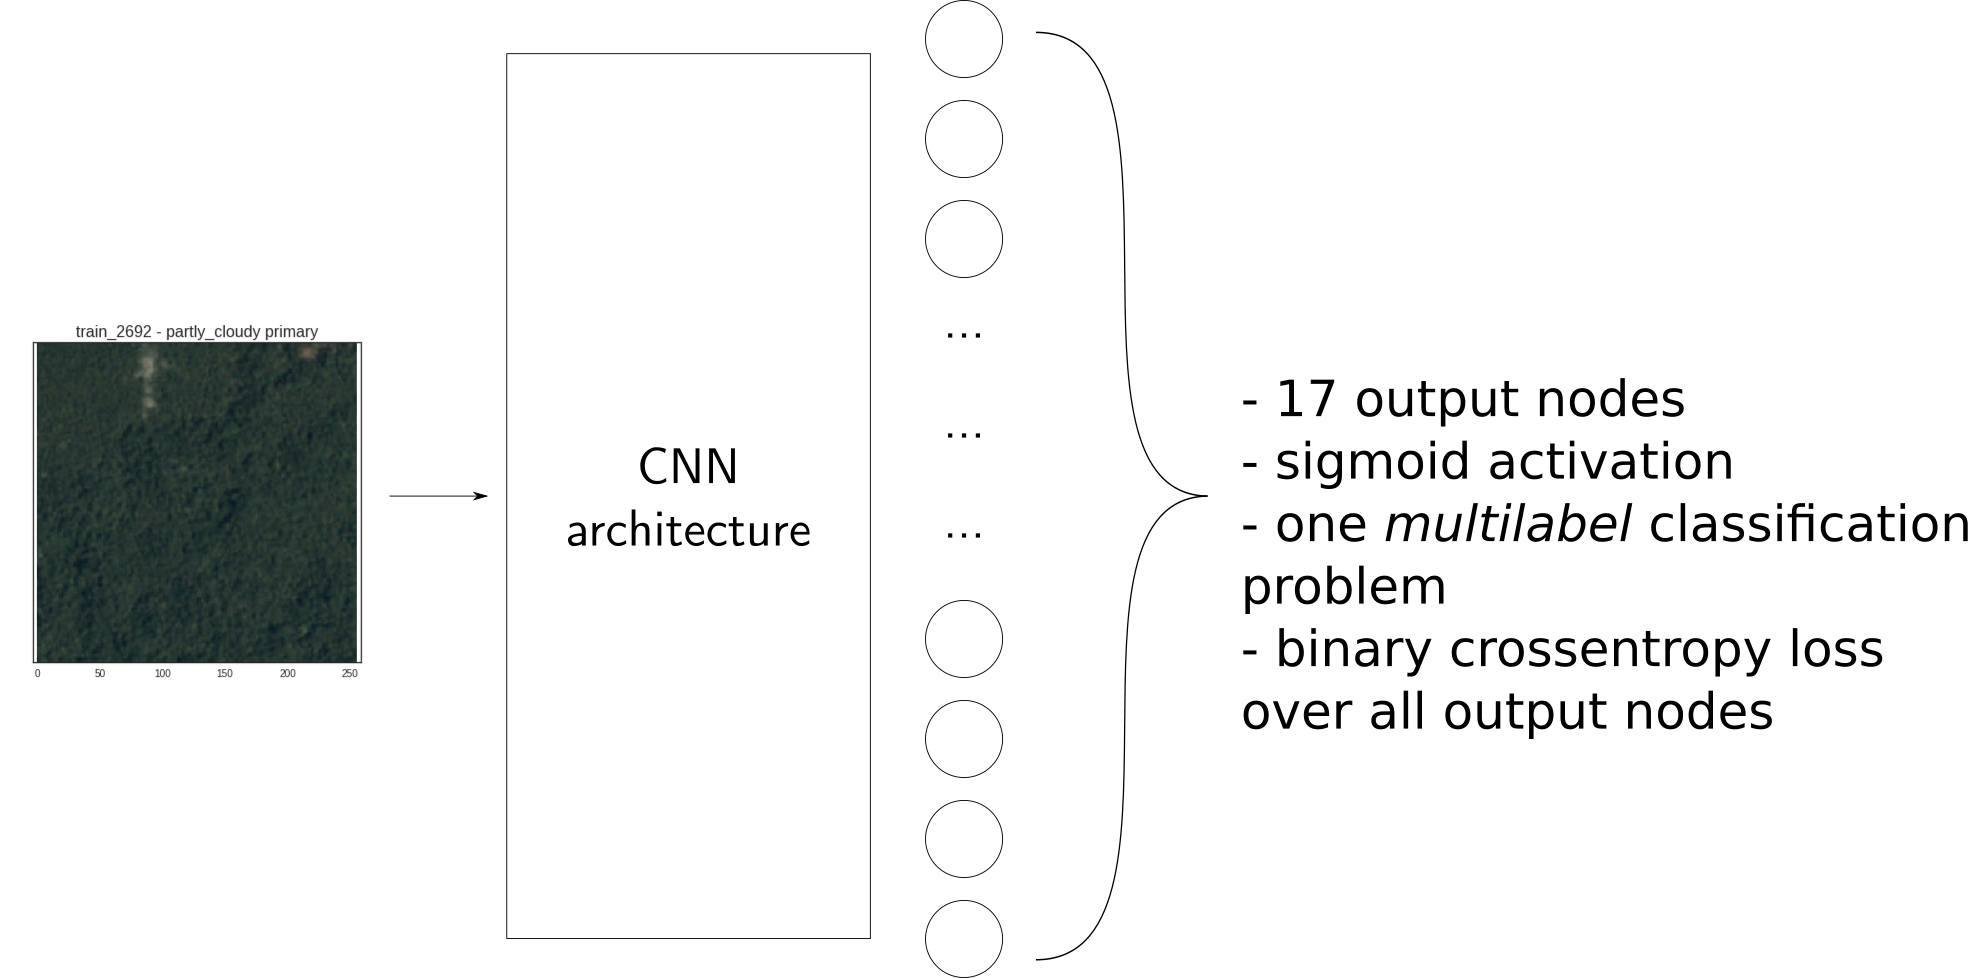
\includegraphics[width=1\linewidth]{figures/GFM1.png}
      \caption{Standard CNN output layer for multiclass labeling of the images.}
   \end{subfigure}
   \begin{subfigure}{0.80\linewidth}
      \centering
      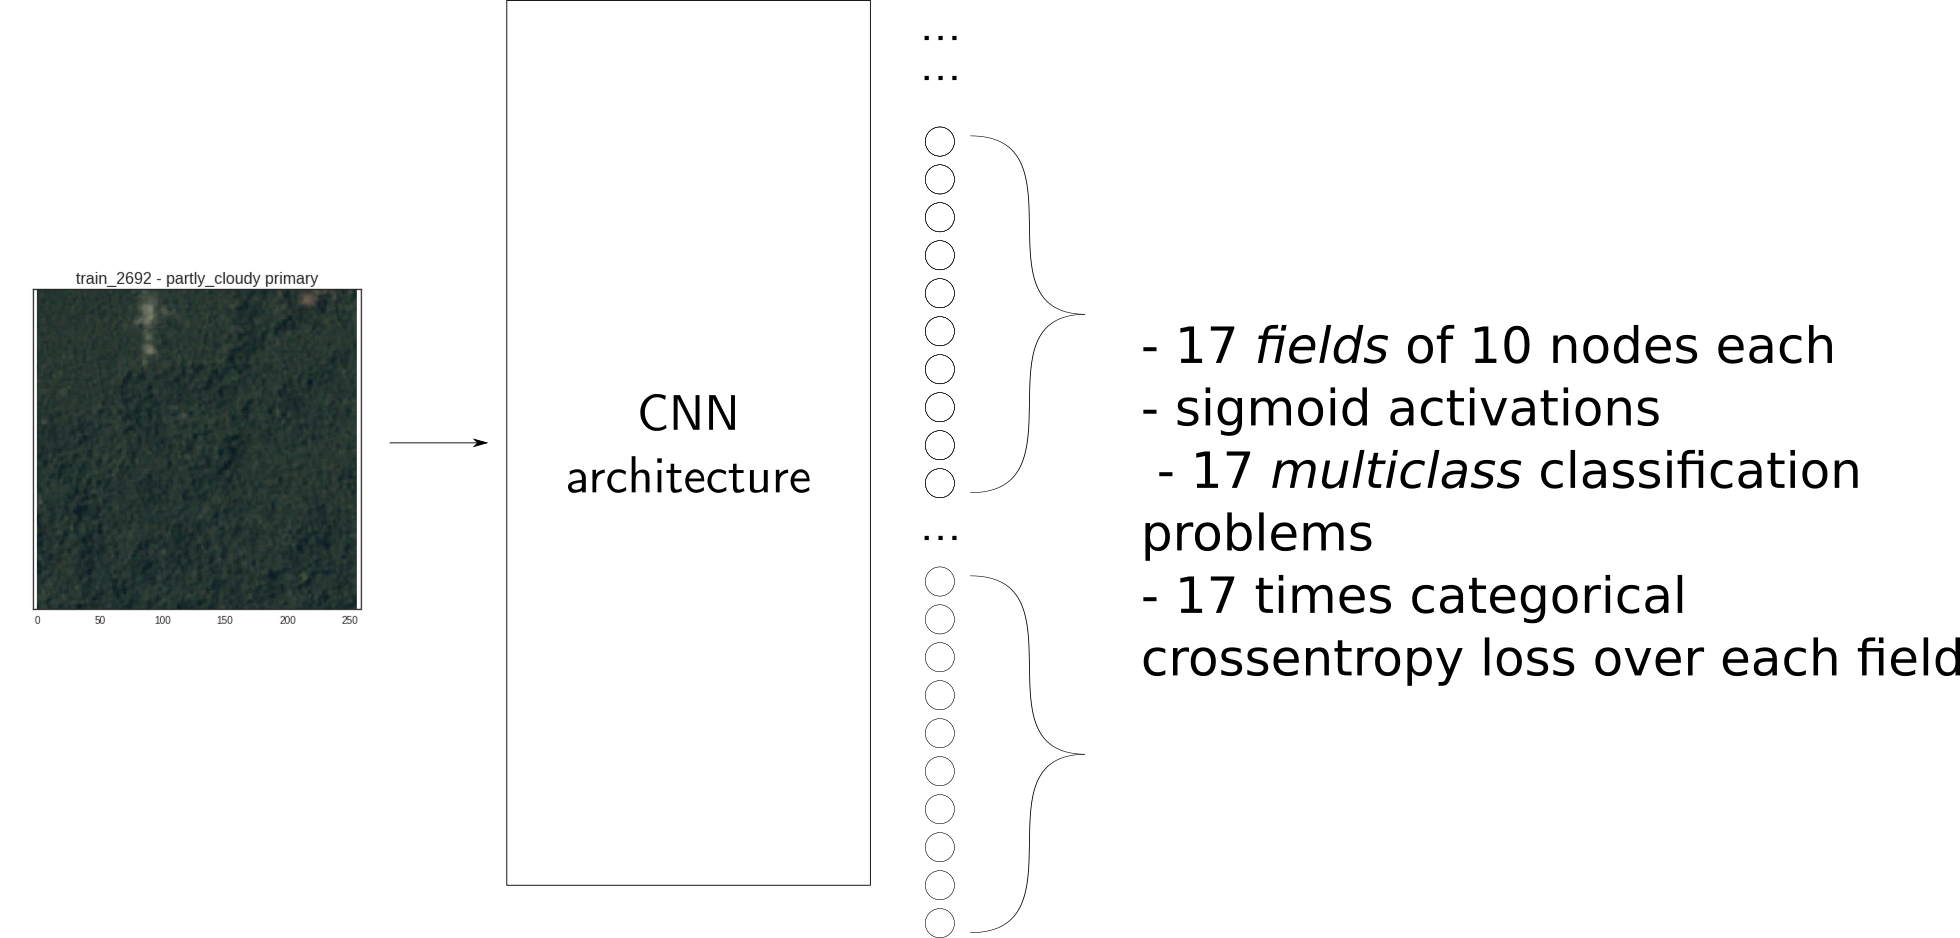
\includegraphics[width=1\linewidth]{figures/GFM2.png}
      \caption{Adapted output to estimate the probabilities required for the GFM.}
   \end{subfigure}
  \caption{Two different CNN output configurations. Top: standard architecture for multiclass labeling. The output layer consists of 17 neurons with a sigmoid output. The model is trained by minimizing a single binary cross-entropy loss over the 17 output nodes. Bottom: the estimate the probabilities required for the GFM algorithm, 17 output fields consisting of 10 nodes each are required. The model is trained by jointly minimizing 17 categorical cross-entropy loss functions, treating each output field as as multi-class classification problem.}
	\label{GFMarchi} 
\end{figure}

\begin{figure}
\centering
   \begin{subfigure}{0.48\linewidth}
      \centering
      \setlength{\fboxsep}{1pt}
      \fbox{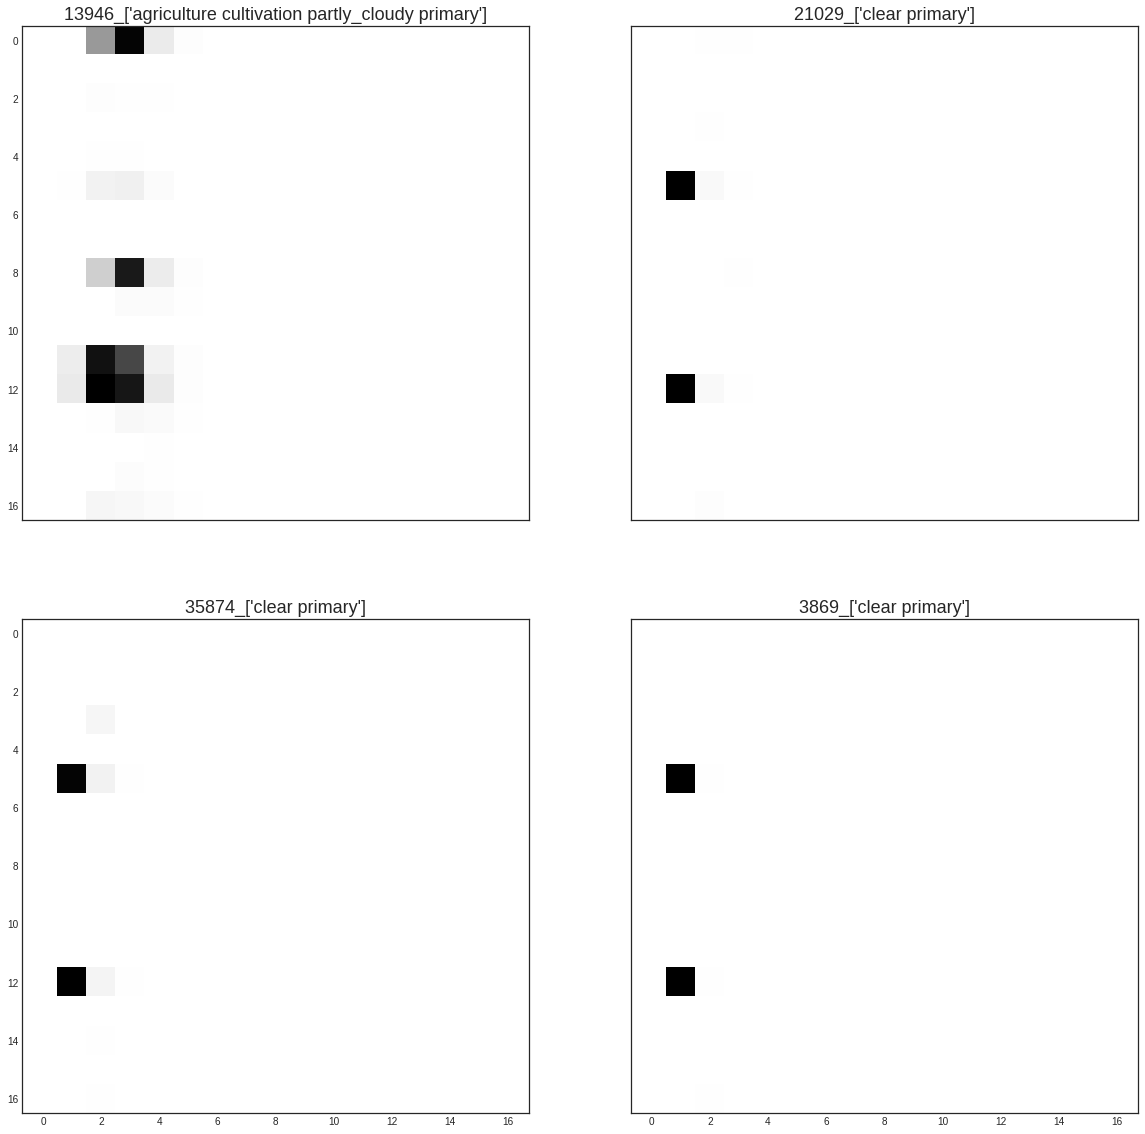
\includegraphics[width=1\linewidth]{figures/P_correct.png}}
      \caption{Matrix $P$ for correct predictions}
   \end{subfigure}
   \begin{subfigure}{0.48\linewidth}
      \centering
      \setlength{\fboxsep}{1pt}%
      \fbox{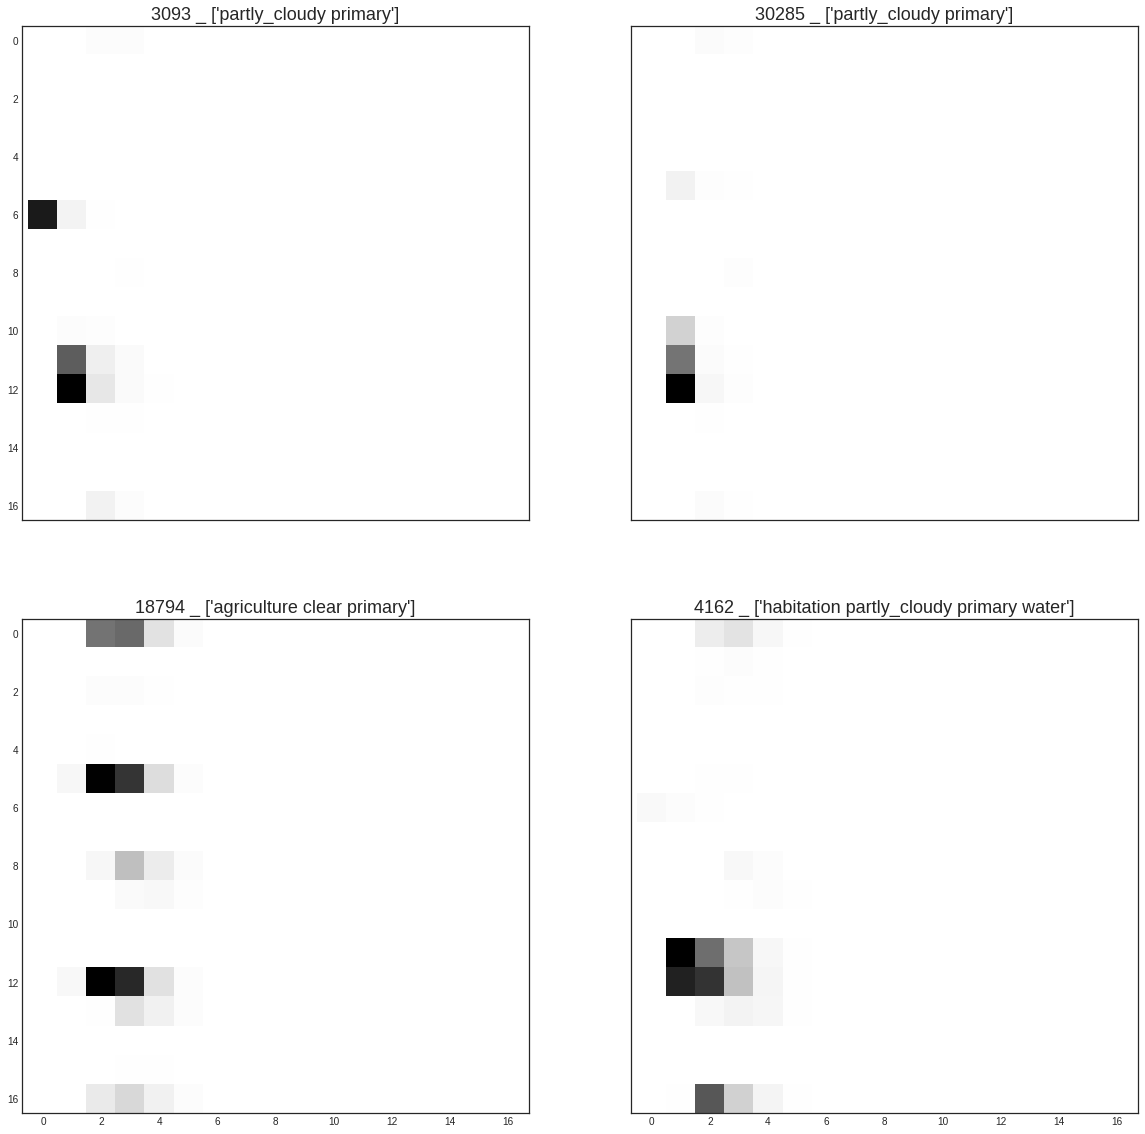
\includegraphics[width=1\linewidth]{figures/P_incorrect.png}}
      \caption{Matrix $P$ for incorrect predictions}
   \end{subfigure}
  \caption{Example outputs of the CNN architecture designed to estimate the matrix $P$. Left: estimated $P$ for correct predictions. Right: estimated $P$ for incorrect predictions. There is clearly more uncertainty for the incorrect predictions. Note that only the first 9 columns of these matrices are actually estimated, the other entries are all zero by default.}
	\label{GFMoutput} 
\end{figure}

\section{Results}

Table \ref{resultstable} summarizes the performance of different individual, non-ensembled models on different image sizes and different strategies for maximizing the F-score. The train and validation scores are the locally obtained scores, and the test score shows the public leaderboard score. In general, using larger images sizes led to better results, although we could obtain decent scores with images as small as 64x64 pixels. Our best individual model was a DenseNet169 architecture where we used pseudo-labeling as well as data augmentation and test-time augmentation. The bottom two models were trained on the entire training data (without validation set), after we had an idea of when to stop training by doing early stopping in other experiments. Using the entire training data set led to an improvement in the $F_2$ score.  

\begin{table}[H]
\centering
\begin{tabular}{c c c c c c }
\textbf{Architecture} & \textbf{Image Size} & \textbf{$F_2$ maximizer} & Train $F_2$& Validation $F_2$ & Test $F_2$\\
\hline
'U-Net' & 64 & thresholding & 0.921 & 0.919 & 0.910 \\
VGG19 & 128 & thresholding  & 0.928 & 0.923 & 0.914 \\
VGG19 & 128 & GFM & 0.928 & 0.926 & 0.923\\
DenseNet169 & 224 & thresholding & 0.936 & / & 0.929 \\
DenseNet169$^*$ & 224 & thresholding & 0.940  & / & \textbf{0.9305} \\
\hline
\footnotesize{$^*$ with pseudo-labeling} & & & & & \\
\end{tabular}
\caption{Performance of individual, non-ensembled models}
\label{resultstable}
\end{table}

Unfortunately, I didn't have the time or resources to run extensive experiments with the GFM method. From the few model runs that were conducted, I can say that the GFM method seemed to suffer a bit more from overfitting that a normal CNN with thresholding. Anyway, there seemed to be no strong competitive advantage in using the GFM method over optimal thresholding, with the GFM method performing slightly better in some settings and worse in other settings. Therefore, we mostly used optimal thresholding towards the end of the competition.


\section{Ensembling and final submission}
Ensembling was done by label-wise majority voting. Because we only stored predictions for the test data, we could not finetune our ensembling on the training data. Instead, we used the following heuristics to select ensemble members: 
\begin{enumerate}
\item{Sort the individual submissions from high to low score on the public LB}
\item{Compute the correlation between these submissions}
\item{Select the highest scoring submission as the first ensemble member}
\item{Loop over the submission files:
\begin{itemize}
\item{If the correlation between the submission and all current members in the ensemble is less than a certain threshold: add the submission to the ensemble}
\end{itemize}}
\item{Use the obtained ensemble for majority voting}
\end{enumerate}

In this way, only the highest scoring and sufficiently uncorrelated submissions were retained. The correlation between two submission files was computed as the number of instances with agreement on all labels divided by the total number of instances. Figure \ref{correlations} shows an example correlation matrix of our submission files with a public LB score larger than 0.927.

\begin{figure}[H]
	\centering
     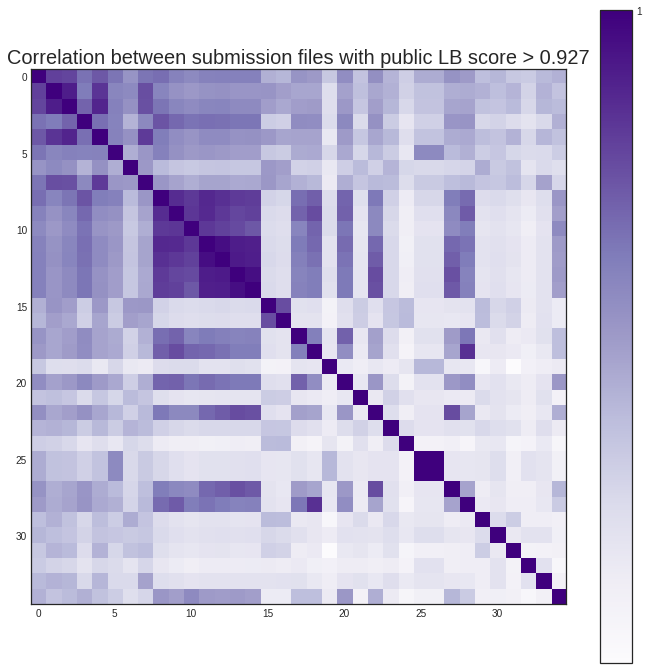
\includegraphics[width=0.7\linewidth]{figures/correlations.png}
	\caption{Correlation matrix for submission files with a public LB score larger than 0.927.}
	\label{correlations} 
\end{figure}

Ensembling significantly increased our public leaderboard score. Our best scoring ensemble on the public board consisted of 15 members and achieved a score of 0.93195. Another ensemble of 9 files achieved a public LB of 0.93193, and this was also our final best private LB score, 0.93063, good for a 41th place in the competition. The winning submission achieved a score of 0.93318 on the private leaderboard.

\section{Conclusions and potential improvements}

The competition turned out to be mostly about finetuning pretrained models and finding a good way to deal with the noisy data by complicated ensembling. I spent quite some time implementing the GFM algorithm on top of a neural network architecture, which in the end did not lead to a competitive advantage over simple threshold optimization. Nevertheless, participating in this competition has learned me a lot about the theory and practice of multi-label classification and convolutional neural networks. I'd like to finish this report with some thoughts on how we could have done better. 

\begin{itemize}
\item{The GFM algorithm did not outperform optimal thresholding and seems to suffer a bit from overfitting. Perhaps some additional regularization on the structure of the matrix $P$ or some modifications to the network architecture for estimating it could help to avoid this problem. I experimented with adding more dropout and reducing the size of the shared layers of the 17 classifiers, but that did not lead to a better score.}
\item{Most top-scoring teams used k-fold cross-validation, whereas we trained each model only once for computational reasons. For sure k-fold cross-validation would have improved our scores.}
\item{We made the mistake not to store our training set predictions, so we had to finetune our ensembling methods on the public leaderboard. Other teams used more advanced ensembling methods and model stacking.}
\item{It's really important to keep good track of hyperparameters, optimizers, small changes to architectures etc. to  keep an overview of which changes could help improving the score, especially since it's so expensive to re-train a large CNN from scratch.}
\item{In the end, me and my colleague had each developed our own extensive body of code, with me working in Keras and my colleague using PyTorch. In future competitions, it would be good to share our code through Github and stick to the same framework to avoid doing the same work twice.}
\end{itemize}

\section*{Appendix}
\begin{figure}[H]
	\centering
     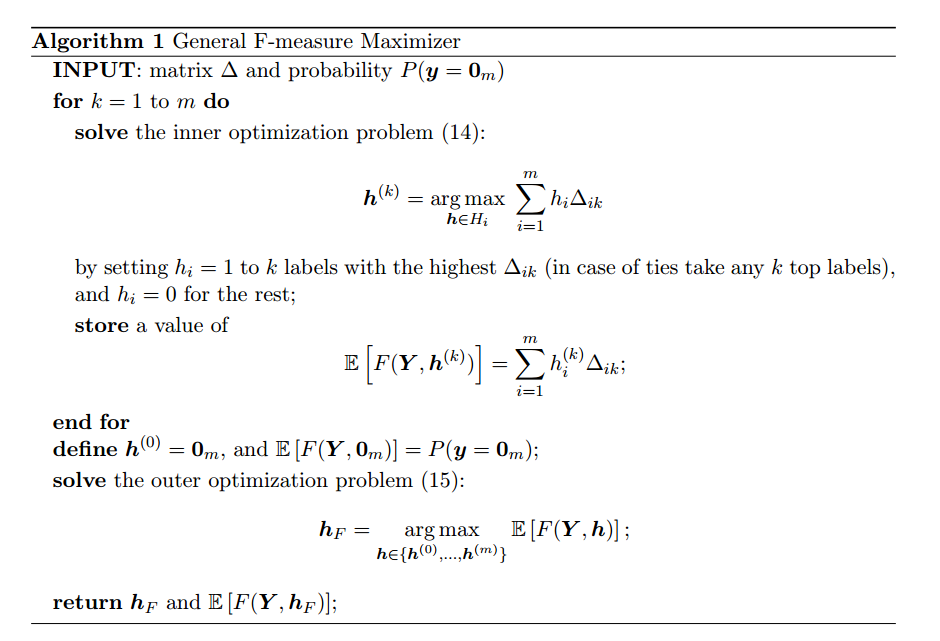
\includegraphics[width=1\linewidth]{figures/GFMalgo.png}
	\caption{Overview of the General F-measure Maximizer algorithm. The input matrix $\Delta$ is equivalent with the matrix $P$ estimated by the proposed CNN architectures in this report. The algorithm is repeated for each instance and $\mathbf{h_F}$ is the Bayes-optimal prediction vector for a particular instance.}
	\label{GFMalgo} 
\end{figure}
\end{document}